
\chapter{Fundamentação Teórica}
\label{fundamentacao-teorica}

\section{Geomarketing}
\label{Geom}
Segundo \citeonline{Sergio2005}, \emph{geomarketing} é o nome dado à área de
gerenciamento de informação que incorpora as dimensões espaciais para auxiliar a
tomada de decisões dentro de um domínio específico de mercado, o que permite
levantar as características de uma determinada região e analisar seu potencial
socioeconômico. Pode ser entendido, assim, como uma ferramenta de análise
estatística de dados, com intuito de localizar padrões que possam ser utilizados
e combinados na elaboração de indicadores, perfis de consumo e estratégias de
negócios, de modo a gerar informação relevante na tomada de decisões.
Geralmente, o serviço é oferecido por consultorias especializadas - o  objetivo
da empresa contratante é a melhoria no desempenho de seu negócio.

\subsection{Relação entre o marketing, geolocalização e estratégias de negócio}
Segundo \citeonline{Cliquet2006}, alguns autores definem o \emph{geomarketing} como uma aplicação específica do espaço econômico, codificando técnicas e divisões geográficas associadas a funções estatísticas. Alguns aspectos espaciais provém ainda características das quais podem ser inferidos novos dados, mais complexos e específicos, a partir de análises mais aprofundadas nos dados iniciais. Este trabalho analítico transforma números em valiosas informações estatísticas, auxiliando na tomada de decisão ao permitir que um gestor visualize de forma mais tangível determinadas situações - por exemplo, projetando estatisticamente cenários positivos ou negativos no futuro do negócio.

Ainda para \citeonline{Cliquet2006}, o espaço geográfico raramente é levado em conta em pesquisas de gestão, exceto quando se trata de escolher a melhor localização para um ponto de vendas ou instalação de uma unidade produtora. No entanto, aspectos espaciais de uma organização são muito mais abrangentes e tem impacto vital no desempenho dos negócios como um todo.

\subsection{Como o geomarketing auxilia e agrega valor ao negócio}
\label{importancia}
O \emph{geomarketing} tem como principal função servir como base de auxílio quando um administrador se depara com questões cruciais para a continuidade dos negócios, sendo de grande importância na definição do público-alvo ou onde estabelecer novas filiais.

Segundo \citeonline{Duarte}, a localização geográfica visualiza de maneira diferenciada as seguintes informações:

\begin{itemize}
  \item Distribuição de unidades e clientes;
  \item Distâncias percorridas no consumo dos clientes;
  \item Padrões de consumo;
  \item Aspectos no entorno das lojas;
  \item Características sociodemográficas;
  \item Pontos interessantes;
  \item Mapear força de vendas;
  \item Localização de prospectos e distribuidores.
\end{itemize}

O grande diferencial em se utilizar o \emph{geomarketing} nos negócios é justamente a eficiência na gestão de informação: transformar dados e números em conhecimento tangível desenvolve a inteligência de uma organização. Sob tal contexto, podemos ainda mencionar que, segundo  \citeonline{Duarte}, o \emph{geomarketing} traz uma enorme valorização nos pontos mencionados abaixo:

\begin{itemize}
  \item Otimiza a rede de negócios e norteia a busca de novos pontos;
  \item Conhece cada loja para análise e comparação;
  \item Estabelece metas;
  \item Ajusta os produtos de cada unidade;
  \item Distribui adequadamente a força em vendas;
  \item Elimina sobreposição de vendedores;
  \item Mede o potencial do mercado;
  \item Analisa a distribuição da concorrência.
\end{itemize}

\subsection{Casos de uso brasileiros}

O termo \emph{geomarketing} ainda não é tão difundido no Brasil, porém cada
vez mais se populariza no âmbito dos negócios: inicialmente, estudos com finalidades geo-estatísticas eram realizados de forma amadora - ao longo dos anos, a super valorização da informação e o desenvolvimento tecnológico fizeram com que a prática evoluísse, juntamente com a especialização de profissionais na área.

Atualmente, o \emph{geomarketing} é parte intrínseca na estratégia de planejamento em organizações brasileiras de todos os tamanhos. Grandes grupos como O Boticário usam largamente o marketing geográfico, assim como pequenas e médias empresas já focam seus sistemas na geolocalização.

Podemos citar como exemplo de aplicação de pequeno negócio um restaurante voltado à alimentação saudável na cidade de Natal - o objetivo do estudo geográfico foi verificar a distribuição de clientes e
mapear áreas de influência para conhecer melhor a demanda do mercado. De acordo
com \citeonline{Seabra2014}, esta investigação permitiu uma compreensão do
fenômeno da área de influência e de variáveis que modelam seu comportamento. O
estudo baseou-se em informações obtidas através de softwares como Google
Maps para o georreferenciamento e análise dos dados - isso só foi possível
graças a fácil disponibilidade e barateamento da tecnologia atual: o
Google Maps é um exemplo de ferramenta de geolocalização bastante popular
e acessível que, há alguns anos, não existia.

O crescimento acelerado de grandes centros urbanos também gerou uma infinidade de aplicações em \emph{geomarketing}, tornando a ferramenta cada vez mais ampla e
complexa - no Brasil, não foi diferente. Um caso de uso a ser citado nesse contexto é a utilização do
\emph{geomarketing} como ferramenta de análise para criação de novas estações na
CPTM (Companhia Paulista de Trens Metropolitanos). Segundo
\citeonline{Mangini2014}, o modelo apresentou ser de grande valia por reduzir de
forma substancial a subjetividade da escolha do local para uma nova estação e
pôde ainda ser utilizado como método para a definição de novas linhas férreas.

Outro caso de uso interessante é o do Shopping Cidade Jardim, em São Paulo, onde em 2016 a empresa Zebra Technologies implantou seu projeto MPact: utilizando redes Wi-Fi/ Bluetooth e oferecendo acesso gratuito à Internet, este captura a localização do cliente em três níveis: zona, posição e presença. Isso permite saber onde ele está, quanto tempo fica em cada setor ou quais produtos está adquirindo, propiciando que varejistas, lojistas e operadores entendam melhor o comportamento dos consumidores. É possível ainda identificar corredores mais cheios, lojas que mais vendem e pontos que recebem maior atenção, auxiliando no monitoramento de vendas. Segundo a \citeonline{zebra}, esta é uma maneira de compreender o que os clientes querem para, assim, ganhá-los e mantê-los.

Diante do exposto nessa seção, podemos perceber a importância do \emph{geomarketing} como
referencial na tomada de decisões estratégicas empresariais, tornando-o hoje uma ferramenta indispensável nos negócios.

\subsection{O tráfego de pessoas no geomarketing}

Segundo \citeonline{Shoppertrak2017}, sem dados de tráfego, estamos apenas tentando adivinhar. Saber quantas pessoas entram numa loja é apenas o início. Quando conhecemos de fato o cliente, percebemos o panorama do que realmente está acontecendo nos negócios.

Conforme \citeonline{Seed2017}, através da contagem de pessoas é possível identificar os períodos de alta e baixa no movimento de clientes ao longo dos horários e dias da semana dentro do estabelecimento. Também é possível calcular a taxa de conversão de negócio, indicando a quantidade de clientes que saíram de uma loja sem efetivar compras.

Ainda para \citeonline{Seed2017}, analisar o fluxo de pessoas permite conhecer o real potencial e aproveitamento do negócio em função do tamanho da loja. Conhecendo o volume de clientes que normalmente ocupa um espaço ao mesmo tempo serve de base para dimensionar a equipe de atendimento, disposição e mix de produtos. Pode-se ainda avaliar a entrada de novos pontos estratégicos de atuação ou mesmo incrementar o alcance nos locais já existentes.

Outros exemplos de dados segundo \citeonline{Seed2017} e \citeonline{Shoppertrak2017} que podem ser inferidos a partir da contagem:

\begin{itemize}
  \item Número de Visitantes por hora;
  \item Horários de pico por baixa;
  \item Comparação de fluxo por horários ou por períodos;
  \item Comparação de performance;
  \item Valor vendas por Número vendas (Ticket médio);
  \item Vendas por Visitantes (Taxa de Conversão);
  \item ROO – Taxa de conversão por ações de marketing;
  \item Determinar custo adicional por cliente e retorno de investimento em marketing;
  \item Escala de funcionários otimizada;
  \item Taxa de atração e tráfego em tempo real.
\end{itemize}

\section{Ferramentas para contagem de pessoas}
Para que o \emph{geomarketing} e o tráfego de pessoas sejam implementados, é necessário medir o número
de pessoas através de uma ferramenta de contagem.

As ferramentas de contagens são sistemas eletrônicos que utilizam leitores para contar as pessoas
\cite{trafsysdef}. O tráfego é gerado por essa contagem durante
certos períodos de tempo. Estes dados, quando aliados a outras métricas de
negócio, geram muitas informações estratégicas.

\subsection{Métodos de contagem}
Não existe apenas um método para contar o número de pessoas. As principais
diferenças entre os contadores estão em: área de cobertura, volume e tecnologia
utilizada. Segundo \citeonline{Ipsos}, os principais meios de
contagem são:

\begin{itemize}
  \item \textbf{Feixes infravermelhos:} são colocados
na entrada de lojas emitindo um feixe infravermelho entre os seus extremos,
quando alguém interrompe o feixe, uma entrada é contada. A área de cobertura é
pequena e o volume de pessoas que ele permite passando pela porta ao mesmo
tempo é baixíssima;
  \item \textbf{Câmeras termais:} o uso de sensores térmicos e
processamento de imagens. Normalmente,
são posicionados no teto para que a imagem capture a temperatura das pessoas
e compare com a do ambiente. Este sistema permite alto volume de tráfego e instalação em entradas complexas;
  \item \textbf{Vídeo:} Utilização de algoritmos complexos, inteligência artificial
   e o processamento de imagens (2D e 3D). A área de cobertura
  pode ser medida de acordo com o uso de câmeras e o volume permitido varia de acordo com os algoritmos;
  \item \textbf{Wi-Fi:} utiliza o receptor Wi-Fi para pegar \emph{frames} únicos de gerenciamento Wi-Fi emitidos por dispositivos
  dentro do alcance. Ideal para áreas onde o volume de pessoas é esparso ou incerto.
\end{itemize}

A escolha de um contador varia de acordo com a complexidade da entrada do lugar, períodos de captura do tráfego de pessoas,
volume de pessoas por período, área de cobertura, precisão desejada, preço, entre outros \cite{trafsys} \cite{Axper2017}.

\subsection{Contagem de pessoas em pesquisas acadêmicas}
Citaremos aqui alguns exemplos de pesquisas acadêmicas focadas em contagem de pessoas. Cada tópico a seguir apresenta um projeto - todos os pesquisadores empregam como ferramentas câmeras de gravação e processamento de imagens. As pesquisas diferenciam-se pelas técnicas de computação utilizadas:

\begin{itemize}

  \item \textbf{Robusto e leve:} com o objetivo de fornecer segurança para ambientes internos o trabalho de \citeonline{Kim2002} preza por um sistema que seja robusto suficiente para garantir as metas, mas não seja tão pesado do ponto de vista de algoritmos e demanda de hardware. O sistema reconhece o movimento de pessoas ao longo de várias direções através de uma única câmera e um processador Pentium IV, assim ele estima e rastreia uma "caixa" ao redor de cada indivíduo para identificá-lo na imagem;

  \item \textbf{Melhora no processamento de imagens e ruídos:} as pesquisas de \citeonline{Luo2016} e \citeonline{Hou2011} consideram a queda de desempenho de sistemas de contagem em ambientes com multidões, oclusões (sombreamento/luminosidade em cada quadro do vídeo) e informações de fundo complexas. O primeiro artigo propõe uma abordagem de cenas \emph{indoor} que leva em conta multidões estacionárias (paradas) ou em movimento. O sistema detecta a multidão e separa os ruídos. Depois, estima-se o número de pessoas através de "ombro-cabeça". Por fim, para reduzir as oclusões, há um filtro que separa quadro por quadro do vídeo e faz um tratamento. Já o segundo, foca em subtrair o fundo, estima o número de pessoas e utiliza técnicas para identificar as pessoas em imagens de baixa resolução;

  \item \textbf{Múltiplos recursos:} os artigos de \citeonline{Venkatesh2015} e \citeonline{Ma2012} consideram múltiplos recursos para contar pessoas em ambientes densos. O primeiro utiliza, principalmente, técnicas matemáticas e técnicas de filtros e imagens para estimar. Já o segundo, utiliza
  múltiplas câmeras e vários níveis de textura para lidar com aparência humana e posições.

\end{itemize}

  As principais caraterísticas em sistemas de contagem que os artigos levantados focaram são: movimentação das pessoas, ambientes de multidão e processamento em tempo real.

\subsection{Produtos empresariais para contagem}
\label{produtos-empresas}
Esta seção descreve exemplos de contadores desenvolvidos por empresas que são mais comumente encontrados no mercado:

\begin{itemize}
\item A empresa Density oferece a contagem a partir de um
dispositivo localizado no topo da entrada que processa imagens 2D \cite{Density2017}, conforme pode ser verificado na \autoref{density}.

\begin{figure}[htb]
  \caption{\label{density}Processamento de imagens 2D - Density People Counter}
  \begin{center}
    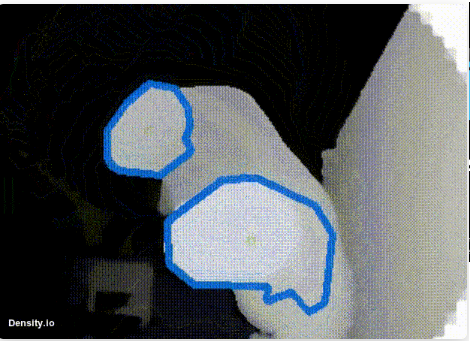
\includegraphics[width=0.40\textwidth]{img/density.png}
  \end{center}
  \legend{Fonte: \citeonline{Density2017}.}
\end{figure}

\item A Axper, além de oferecer o processamento de imagens 2D, como a Density, disponibiliza também um dispositivo que processa imagens em 3D, realizando a cobertura de todo o ambiente \cite{Axper2017}, como pode ser visto na \autoref{axper}.

\begin{figure}[htb]
  \caption{\label{axper}Processamento de imagens 2D e 3D - Axper People Counter}
  \begin{center}
    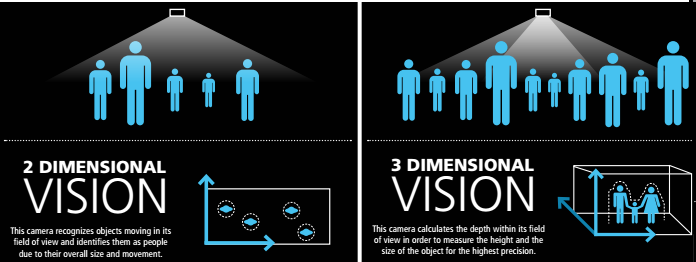
\includegraphics[width=0.70\textwidth]{img/axper.png}
  \end{center}
  \legend{Fonte: \citeonline{Axper2017}.}
\end{figure}

\item A \citeonline{V-Count2017} oferece soluções de contagem a partir de imagens termais e sinais Wi-Fi. Na \autoref{v-count1}, a contagem ocorre por um
aparelho que, fixado na entrada da loja, capta sinais emitidos pelos dispositivos móveis pertencentes  às pessoas que transitam dentro da área coberta. Já a \autoref{v-count2} mostra as soluções que processam imagens e a temperatura para identificar os clientes e seus hábitos.

\begin{figure}[htb]
  \caption{\label{v-count1}Street Counting - V-Counter}
  \begin{center}
    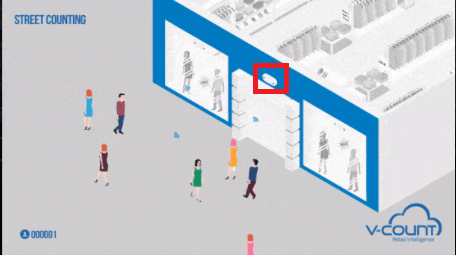
\includegraphics[width=0.70\textwidth]{img/v-count.png}
  \end{center}
  \legend{Fonte: \citeonline{V-Count2017}.}
\end{figure}

\begin{figure}[htb]
  \caption{\label{v-count2}Visitor Counting e Camera Heatmap - V-Counter}
  \begin{center}
    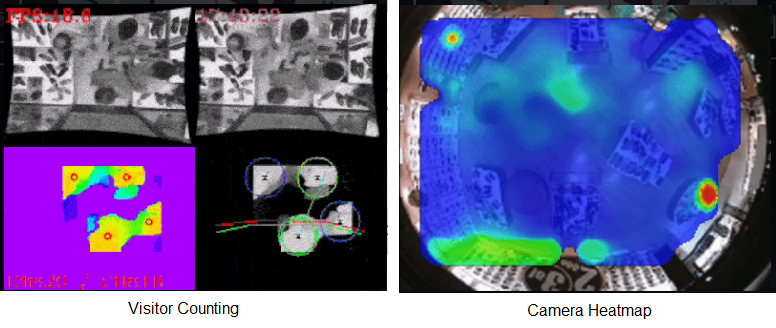
\includegraphics[width=0.70\textwidth]{img/termal-vcount.png}
  \end{center}
  \legend{Fonte: \citeonline{V-Count2017}.}
\end{figure}

\end{itemize}

%\subsection{Motivos de adoção} ISSo AQUI VAMOS COLOCAR DEPOIS SE NÃO NAO DÀ TEMPO
%Os motivos que levam uma organização a adotar as ferramentas de contagem de pessoas são:
\subsection{Escolha do método de contagem}
Foi observado que as principais pesquisas de técnicas para a contagem de pessoas abordam o processamento de imagens e vídeo. Já no âmbito empresarial,
há diversificadas soluções partindo desde o uso dessas imagens até o uso de emissão de sinais Wi-Fi.
As soluções em TI que empregam as redes sem fio para identificar pessoas são variadas. Por exemplo,
uma área amplamente explorada em pesquisas é a localização de pessoas em
ambientes fechados (\emph{indoor location}) que utiliza dispositivos móveis e emissão de sinais \emph{wireless} \cite{Ferreira2016}
\cite{Puhl2016} \cite{Figuera2011}. No entanto, o uso da técnica de contagem por Wi-Fi como ferramenta do \emph{geomarketing} não é amplamente desenvolvida na comunidade aberta, permanecendo restrita a empresas de consultoria e serviços de TI, como citadas na \autoref{produtos-empresas}.

Devido à grande área de cobertura na tecnologia Wi-Fi e à baixa exploração de seu uso como ferramenta de \emph{geomarketing} em comunidade aberta, o presente trabalho priorizou esse tipo de comunicação para a medição do tráfego de pessoas. A escolha considerou ainda o fato de que a identificação de indivíduos em multidões foi apontada como tendência de pesquisa.


\section{Dispositivos móveis}

\subsection{Número e uso de dispositivos}

Hoje em dia, é muito difícil encontrar nas ruas uma pessoa que não esteja portando qualquer tipo de dispositivo móvel com acesso à rede - essa proliferação, segundo diversas estimativas abaixo apresentadas, só tende a aumentar - isso torna o uso de redes de internet e aparelhos móveis uma fonte para exploração em \emph{geomarketing} cada vez mais importante:
\begin{itemize}
\item A \citeonline {Gartner2014} calculou que, até o final de 2016, possuíamos 6,4 bilhões de dispositivos conectados à internet no mundo inteiro, prevendo que em 2020 serão 20.8 milhões de aparelhos em atividade.
\item A \citeonline{Ciscoblogs} estimou que, até 2013, havia 80 dispositivos se conectando na Internet por segundo - em 2020, estima-se que atingiremos 250 aparelhos acessando a rede por segundo e existirão, em média, 50 bilhões de dispositivos ativos.
\end{itemize}

Abaixo, a \autoref{cisco2011} apresenta estimativas de que, até 2020, teremos quase 7 aparelhos conectados por pessoa:

\begin{figure}[htb]
  \caption{\label{cisco2011}Número de dispositivos conectados - Cisco IBSG 2011}
  \begin{center}
    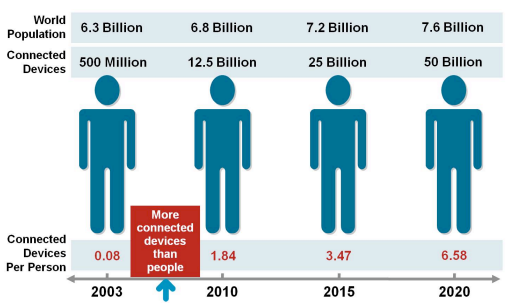
\includegraphics[width=0.70\textwidth]{img/cisco-2011.png}
  \end{center}
  \legend{Fonte: \citeonline{Evans2011}.}
\end{figure}

Apesar da expressiva diferença entre as estimativas anteriores, é bastante perceptível o crescimento no uso da rede em dispositivos móveis. A pesquisa da \citeonline{Cisco2017a} mostra o aumento do tráfego de dados nos tipos aparelhos mais utilizados, como pode ser visto na \autoref{cisco-2017}. De 2016 até 2021, a elevação em consumo de exabytes por mês se destaca entre os \emph{smartphones}.

\begin{figure}[htb]
  \caption{\label{cisco-2017}Tráfego mundial de dispositivos móveis por tipo}
  \begin{center}
    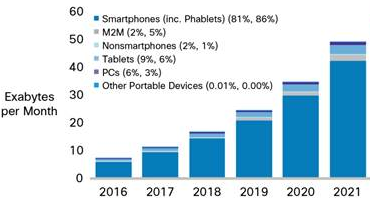
\includegraphics[width=0.70\textwidth]{img/cisco-2017.png}
  \end{center}
  \legend{Fonte: \citeonline{Cisco2017a}.}
\end{figure}

No Brasil, segundo a \citeonline{Teleco}, a pesquisa da IDC no último trimestre de 2016 calculou que foram vendidos 48,4 milhões de dispositivos no país, sendo 4,9 milhões de celulares tradicionais e 43,5 milhões de \emph{smartphones} - apesar da queda nos últimos anos, a proporção em vendas ainda é maior para aparelhos do tipo \emph{smartphone}.

Já o total de celulares, em março de 2017, era de aproximadamente 242 milhões, como demonstra a \autoref{dados2017}.

\begin{figure}[!h]
  \caption{\label{dados2017}Quantidade de Celulares no Brasil - Março 2017}
  \begin{center}
    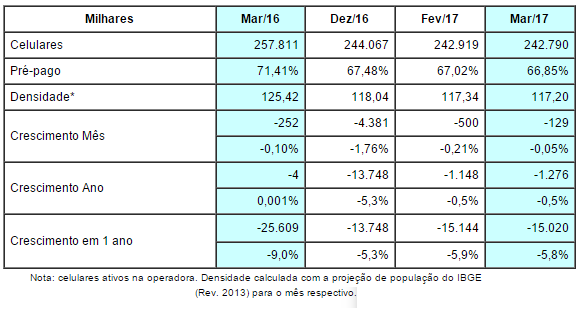
\includegraphics[width=0.7\textwidth]{img/dados2017.png}
  \end{center}
  \legend{Fonte: \citeonline{Teleco}.}
\end{figure}

\subsection{Dispositivo móvel como objeto identificador}
\label{dispositivo-coisa}
Assim como os RFIDs passivos utilizados em uma cadeia de suprimentos para identificar produtos que vão num caminhão, ou como os códigos de barras
que fornecem ao operador de caixa informações sobre um produto, os dispositivos móveis, como os \emph{smartphones}, serão utilizados
como objetos identificadores neste trabalho. Tendo em vista que a proporção de \emph{smartphones} é maior que a de celulares tradicionais no Brasil e, em
todo o mundo, considera-se esse equipamento de uso comum. Além disso, esses dispositivos móveis fornecem informação pública passiva
através da rede Wi-Fi e independem da fabricante para serem detectados numa rede - serão utilizados como meio
de identificação das pessoas.

\subsection{Exemplos em detecção de dispositivos através de redes Wi-Fi}
\label{trabalhos-correlatos}
Este subcapítulo apresenta alguns trabalhos que empregam a detecção de dispositivos móveis por sinais de Wi-Fi, utilizando-os como ferramenta de \emph{geomarketing}.

\begin{itemize}
\item Meshlium Xtreme: trata-se de um produto da empresa Libelium que detecta dispositivos  móveis e veículos através de sinais Wi-Fi e Bluetooth, visando otimizar a inteligência nos negócios. O sistema conta pessoas e automóveis, gerando informações \cite{libelium} como: quantidade de pessoas passando numa mesma rua diariamente, o tempo médio em que permanecem nela, diferenciação entre indivíduos visitantes ou residentes (moradores da região), rotas caminhadas entre lojas, número de veículos em tempo real, o tempo médio que um veículo fica parado, a sua velocidade média e, quando um congestionamento é detectado, o tempo gasto em rotas alternativas.

Os dispositivos móveis não precisam estar conectados a qualquer AP para serem detectados, e podem ser manufaturados por qualquer fabricante. Os veículos são identificados dentro de velocidades até 100 km/h. O objetivo do produto é medir a quantidade de pessoas e carros em determinado ponto e hora específica, possibilitando criar estratégias de negócios com respeito ao tráfego de indivíduos e carros na área designada. As figuras
\autoref{meshlium-celulares} e \autoref{meshlium-carros} demonstram o
funcionamento do produto.

\begin{figure}[htb]
  \caption{\label{meshlium-celulares}Detecção de \emph{smartphones}}
  \begin{center}
    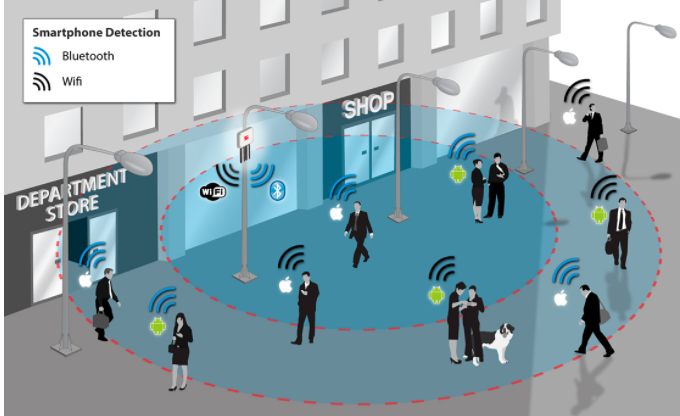
\includegraphics[width=0.60\textwidth]{img/meshlium-celulares.png}
  \end{center}
  \legend{Fonte: \citeonline{libelium}.}
\end{figure}

\begin{figure}[htb]
  \caption{\label{meshlium-carros}Detecção de veículos}
  \begin{center}
    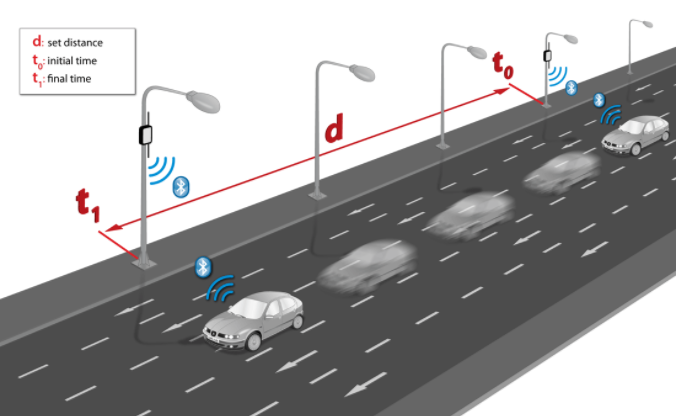
\includegraphics[width=0.60\textwidth]{img/meshlium-carros.png}
  \end{center}
  \legend{Fonte: \citeonline{libelium}.}
\end{figure}

\item {How many people are around}
``How many people are around'' (em português: quantas pessoas estão ao redor) é um projeto encontrado no Github do usuário \citeonline{Schollz2017}, que utiliza um \emph{cluster} de Raspberry Pi's para calcular o número de pessoas próximas e/ou dentro de casa. Para tanto, ele utiliza o protocolo de análise Tshark para detectar Wi-Fi \emph{probe requests} de \emph{smartphones} e a linguagem Python. Além disso, os dados capturados podem ser visualizados em forma de gráfico.

\end{itemize}
